\documentclass{article}

\usepackage{fancyhdr}
\usepackage{extramarks}
\usepackage{amsmath}
\usepackage{amsthm}
\usepackage{amsfonts}
\usepackage{tikz}
\usepackage[plain]{algorithm}
\usepackage{algpseudocode}
\usepackage{enumerate}
\usepackage{graphicx}
\usepackage{pythonhighlight}
\usepackage{amssymb}

\usetikzlibrary{automata,positioning}

%
% Basic Document Settings
%  

\topmargin=-0.45in
\evensidemargin=0in
\oddsidemargin=0in
\textwidth=6.5in
\textheight=9.0in
\headsep=0.25in

\linespread{1.1}

\pagestyle{fancy}
\lhead{\hmwkAuthorName}
\chead{\hmwkClass\ (\hmwkClassInstructor): \hmwkTitle}
\rhead{\firstxmark}
\lfoot{\lastxmark}
\cfoot{\thepage}

\renewcommand\headrulewidth{0.4pt}
\renewcommand\footrulewidth{0.4pt}

\setlength\parindent{0pt}

%
% Create Problem Sections
%

\newcommand{\enterProblemHeader}[1]{
    \nobreak\extramarks{}{Problem \arabic{#1} continued on next page\ldots}\nobreak{}
    \nobreak\extramarks{Problem \arabic{#1} (continued)}{Problem \arabic{#1} continued on next page\ldots}\nobreak{}
}

\newcommand{\exitProblemHeader}[1]{
    \nobreak\extramarks{Problem \arabic{#1} (continued)}{Problem \arabic{#1} continued on next page\ldots}\nobreak{}
    \stepcounter{#1}
    \nobreak\extramarks{Problem \arabic{#1}}{}\nobreak{}
}

\setcounter{secnumdepth}{0}
\newcounter{partCounter}
\newcounter{homeworkProblemCounter}
\setcounter{homeworkProblemCounter}{1}
\nobreak\extramarks{Problem \arabic{homeworkProblemCounter}}{}\nobreak{}

%
% Homework Problem Environment
%
% This environment takes an optional argument. When given, it will adjust the
% problem counter. This is useful for when the problems given for your
% assignment aren't sequential. See the last 3 problems of this template for an
% example.
%
\newenvironment{homeworkProblem}[1][-1]{
    \ifnum#1>0
        \setcounter{homeworkProblemCounter}{#1}
    \fi
    \section{Problem \arabic{homeworkProblemCounter}}
    \setcounter{partCounter}{1}
    \enterProblemHeader{homeworkProblemCounter}
}{
    \exitProblemHeader{homeworkProblemCounter}
}

%
% Homework Details
%   - Title
%   - Due date
%   - Class
%   - Section/Time
%   - Instructor
%   - Author
%

\newcommand{\hmwkTitle}{Homework\ \#1}
\newcommand{\hmwkDueDate}{March 22, 2020}
\newcommand{\hmwkClass}{Reinforcement Learning}
\newcommand{\hmwkClassInstructor}{Professor Ziyu Shao}
\newcommand{\hmwkAuthorName}{Tianyuan Wu}
\newcommand{\hmwkAuthorID}{63305667}

%
% Title Page
%

\title{
    \vspace{2in}
    \textmd{\textbf{\hmwkClass:\ \hmwkTitle}}\\
    \normalsize\vspace{0.1in}\small{Due\ on\ \hmwkDueDate\ at 11:59pm}\\
    \vspace{0.1in}\large{\textit{\hmwkClassInstructor}}
    \vspace{3in}
}

\author{\textbf{\hmwkAuthorName}\\ \hmwkAuthorID}
\date{}

\renewcommand{\part}[1]{\textbf{\large Part \Alph{partCounter}}\stepcounter{partCounter}\\}

%
% Various Helper Commands
%

% Useful for algorithms
\newcommand{\alg}[1]{\textsc{\bfseries \footnotesize #1}}

% For derivatives
\newcommand{\deriv}[1]{\frac{\mathrm{d}}{\mathrm{d}x} (#1)}

% For partial derivatives
\newcommand{\pderiv}[2]{\frac{\partial}{\partial #1} (#2)}

% Integral dx
\newcommand{\dx}{\mathrm{d}x}

% Alias for the Solution section header
\newcommand{\solution}{\textbf{\large Solution}}

% Probability commands: Expectation, Variance, Covariance, Bias
\newcommand{\E}{\mathrm{E}}
\newcommand{\Var}{\mathrm{Var}}
\newcommand{\Cov}{\mathrm{Cov}}
\newcommand{\Bias}{\mathrm{Bias}}

\begin{document}

\maketitle

\pagebreak

\begin{homeworkProblem}
    Sampling from probability distributions. Show histograms and compare them to corresponding PDF.
    \\
    \\
    \textbf{Solution}
    \begin{itemize}
        \item [1)] 
            Sampling from the Logistic distribution by using Unif(0,1).\\
            The CDF of Logistic distribution is: $F(x) = \frac{e^x}{1+e^x}$
            So we can use inverse transform technique and find the inversion of it,
            which is $F^{-1}(u) = \log{\frac{u}{1-u}}$. So for each sample, we generate a uniform
            distributed r.v. and return the inversion of it. The python code is shown below.
            \begin{python}
                def logistic():
                    u = uniform(0, 1)
                    return log(u/(1-u))
            \end{python}
            Also, we can find the PDF of the logistic distribution is $f(x) = \frac{e^{-x}}{(1+e^{-x})^2}$
            Based on these analysis, I generate 200,000 sample and draw the histogram and PDF shown in Fig.1.
            \begin{figure}[H]
                \centering
                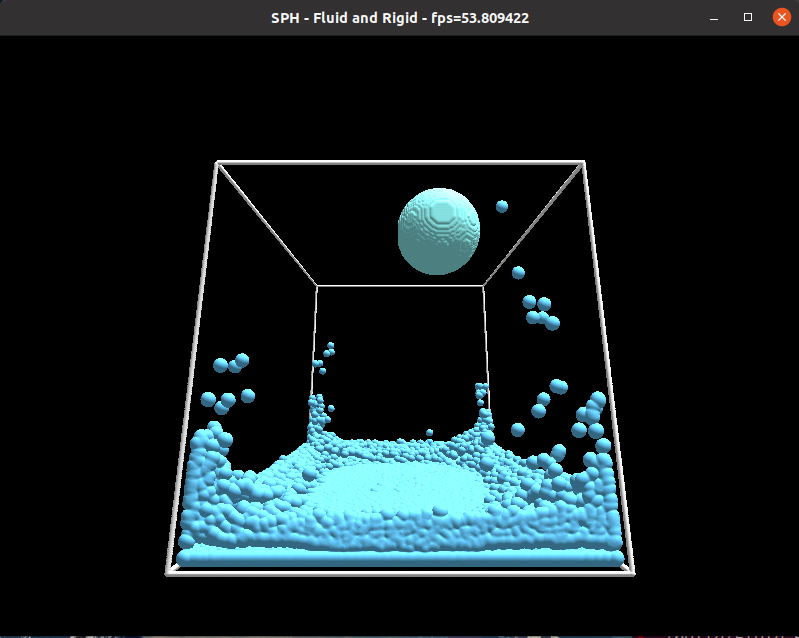
\includegraphics[scale=0.32]{/Users/wuty/Desktop/temp/si252/hw1/p1/1.png}
                \caption{Logistic distribution via inverse transform}
            \end{figure}
        \item [2)]
            Sampling from the Rayleigh distribution by using Unif (0,1).\\
            The CDF of Logistic distribution is: $F(x) = 1-e^{-\frac{x^2}{2}}$. so we can also
            use the inverse transform to find $F^{-1}(u) = \sqrt{-2\log{(1-u)}}$
            \begin{python}
                def rayleigh():
                    u = uniform(0, 1)
                    return sqrt(-2*log(1-u))
            \end{python}
            Also, we can find the PDF of the logistic distribution is $f(x) = xe^{\frac{-x^2}{2}}$
            Based on these analysis, I generate 200,000 sample and draw the histogram and PDF shown in Fig.2.
            \begin{figure}[H]
                \centering
                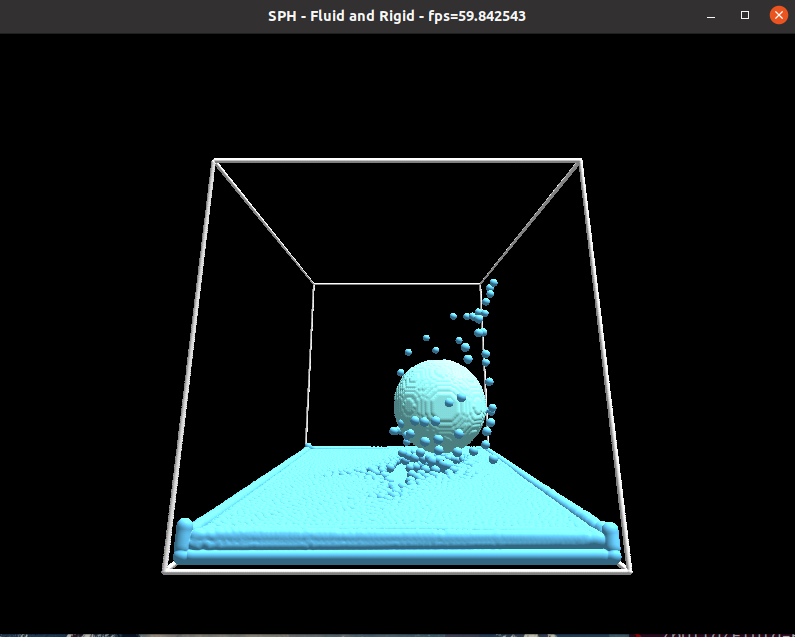
\includegraphics[scale=0.32]{/Users/wuty/Desktop/temp/si252/hw1/p1/2.png}
                \caption{Rayleigh distribution via inverse transform}
            \end{figure}
        \item [3)]
            Sampling from the standard Normal distribution with both the Box-Muller method and the Acceptance-Rejection 
            method. Compare the pros and cons of both methods.
            \begin{itemize}
                \item [1.] Box-Muller method\\
                    First, generate two r.v. $u_1 \sim U(0,\ 1)$ and $u_2 \sim U(0, 1)$.\\
                    Then, by the Box-Muller method, $n_1 = \sqrt{-2\log(u_1)}*\cos(2\pi u_2)$ and  
                    $n_2 = \sqrt{-2\log(u_1)}*\sin(2\pi u_2)$ are 2 independent $r.v.$ which both obey normal distribution.
                    \begin{python}
                    def normal():
                        u1 = uniform(0,1)
                        u2 = uniform(0,1)
                        return sqrt(-2*log(u1))*cos(2*pi*u2)
                    \end{python}
                    The result is shown in Fig.3
                    \begin{figure}[H]
                        \centering
                        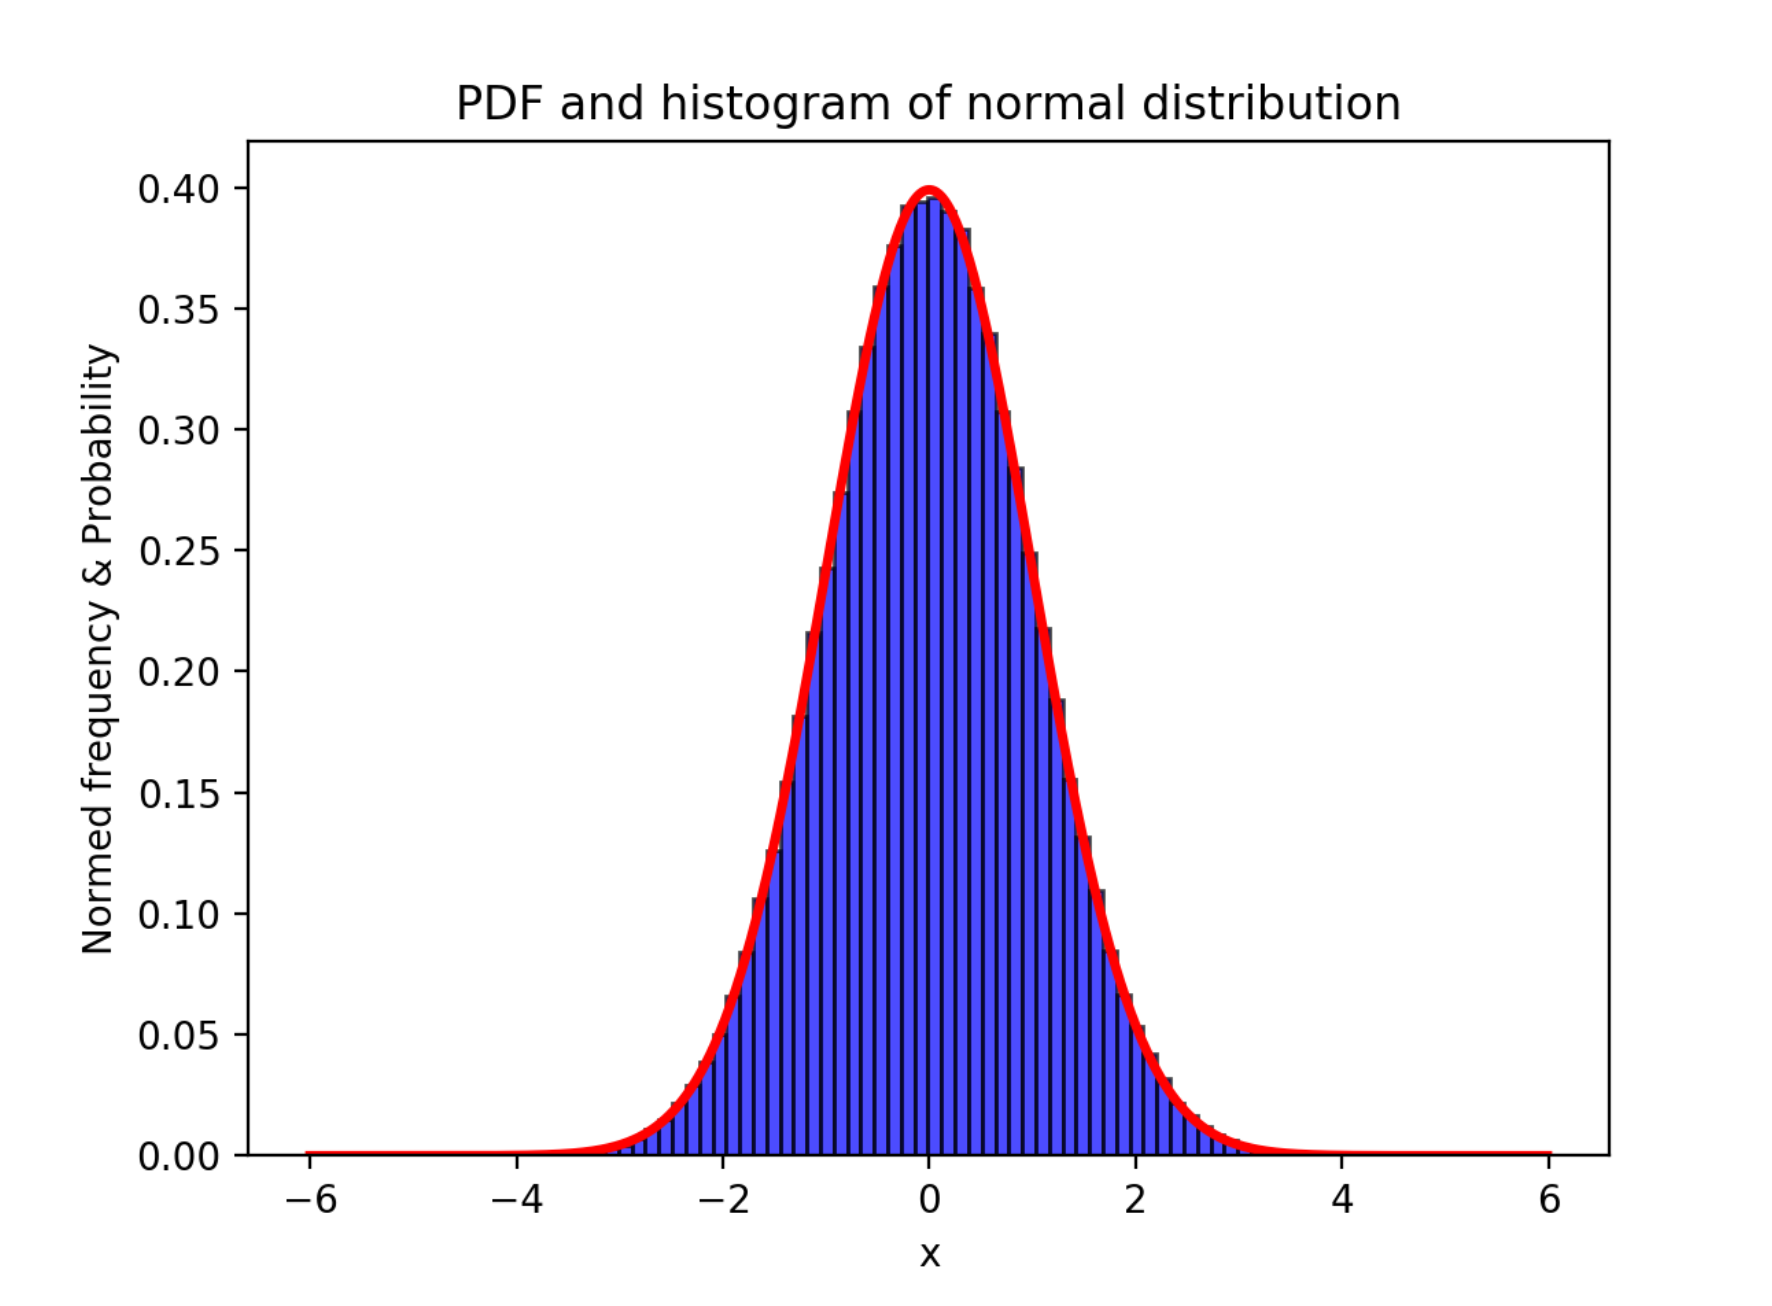
\includegraphics[scale=0.32]{/Users/wuty/Desktop/temp/si252/hw1/p1/3.png}
                        \caption{Normal distribution via Box-Muller method}
                    \end{figure} 
                \item [2.] Acceptance-Rejection method\\
                    First, we can generate a standard exponential distribution $q(x) \sim Expo(1)$ by inverse transform method.\\
                    Second, let $Z \sim \frac{2}{\sqrt{2\pi}}e^{-\frac{x^2}{2}} = p(x)$ which is half of the normal distribution.\\
                    Then, find $c = sup_{\epsilon}{\frac{q(\epsilon)}{p(\epsilon)}}$, which equals to $\sqrt{\frac{2e}{\pi}}$\\
                    Finally, run the Acceptance-Rejection method, generate $y$ from $q(x)$, and $u$ from $U(0,\ 1)$. Accepts when
                    $u \textless \frac{p(y)}{cq(y)}$. The python code is:
                    \begin{python}
                    def normal_acc_rej():
                        def expo_1():
                            u = uniform(0, 1)
                            return -log(u)
                        y = expo_1()
                        u = uniform(0, 1)
                        if u < exp(-0.5*(y-1)**2):
                            return y if random() < 0.5 else -y
                        return normal_acc_rej()
                    \end{python}
                    The result is shown in Fig.4
                    \begin{figure}[H]
                        \centering
                        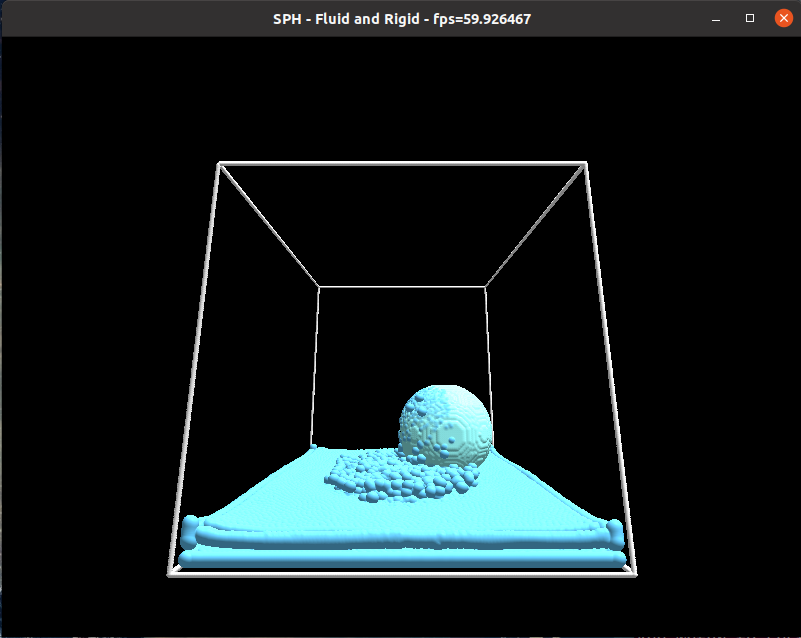
\includegraphics[scale=0.32]{/Users/wuty/Desktop/temp/si252/hw1/p1/4.png}
                        \caption{Normal distribution via Box-Muller method}
                    \end{figure} 
                \item [3.] Comparison\\
                    The results of 2 methods shown above are quite similar when $N=200,000$. But the Box-Muller method
                    may be more efficient, because Acceptance-Rejection method may reject many times 
                    when $u \ge \frac{p(y)}{cq(y)}$ .
                    Then, the recursive run of sampling code will take a lot of time.
            \end{itemize}
        \item [4)] Sampling from the Beta distribution (you can use any method introduced in our class).
            To sample from the Beta distribution from uniform distribution, I considered 2 different cases.
            \begin{itemize}
                \item [1.] a, b greater than 1, and $a, b \in \mathbb{Z}^+$ \\
                    We can refer to the relationship between beta distribution and order statistics.
                    Notice that $u_j \sim Beta(j, n-j+1)$, then we can find the parameters $n, j$ in order statistics
                    can be represented by $a,\ b$ as $j=a$ and $n=a+b-1$. We can just create $n$ i.i.d random variables which 
                    obey $U(0,\ 1)$, sort them and find $j^{th}$ minimum of the sequence.
                \item [2.] Otherwise \\
                    Notice that $Beta(a, b) = \frac{\Gamma(a)\Gamma(b)}{\Gamma(a+b)}$, where $\Gamma(x)$ is the 
                    standard gamma distribution $\Gamma(x, 1)$.\\
                    We can use Acceptance-Rejection method to get the result for gamma distribution, and combine them 
                    to sample from beta distribution.
            \end{itemize}
            The python code is shown below:
            \begin{python}
                def beta(*args):
                    assert(len(args) == 2)
                    a, b = args[0], args[1]
                    def order_stat(_n, _j):
                        l = sorted([uniform(0,1) for _ in range(_n)])
                        return l[_j-1]
                    def beta_int(_a, _b):
                        return order_stat(_a+_b-1, _a)
                    if a < 1 and b < 1:
                        u1, u2 = uniform(0, 1), uniform(0, 1)
                        x = u1**(1/a); y = u2**(1/b)
                        if x + y < 1:
                            return x/(x+y)
                        return beta(a, b)
                    else:
                        return beta_int(a, b) 
            \end{python}
            For the PDFs, I use numeric integral to caculate $\beta(a, b)$:
            \begin{python}
                def beta_integral(a, b):
                    I, dx = 0, 0.001
                    for i in np.arange(0.001, 1, dx):
                        I += (i**(a-1))*((1-i)**(b-1))*dx
                    return I
            \end{python}
            The function is tested under different cases: $Beta(0.5, 0.5)$, $Beta(2, 8)$, $Beta(1, 1)$ and $Beta(5, 5)$, 
            all of these results are shown in Fig.5.
            \begin{figure}[H]
                \centering
                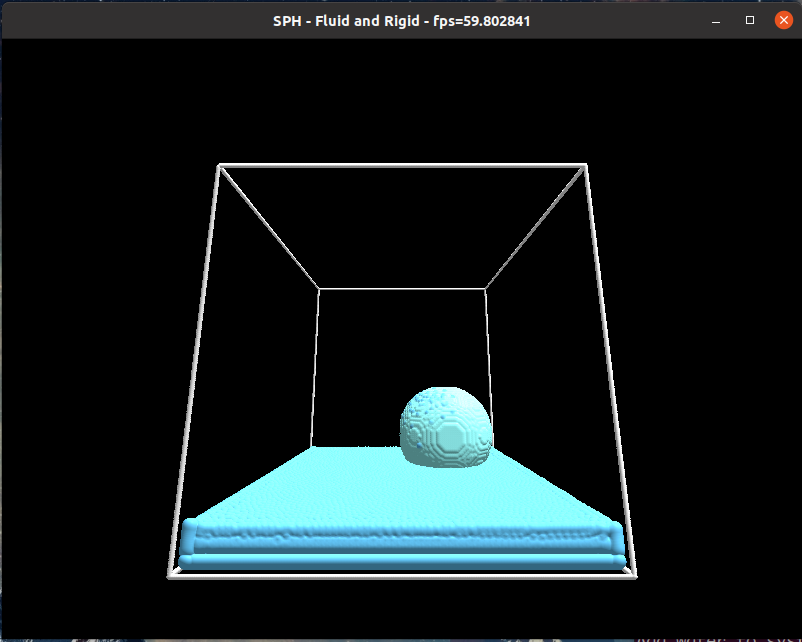
\includegraphics[scale=0.4]{/Users/wuty/Desktop/temp/si252/hw1/p1/5.png}
                \caption{Beta distribution under different parameters}
            \end{figure} 
    \end{itemize}
\end{homeworkProblem}


\begin{homeworkProblem}
    Given a random variable $X \sim N (0,\ 1)$, evaluate the tail probability $P(X > 8)$ \\
    (a) Use the standard sample average method. \\
    (b) Use the importance sampling method. \\
    \textbf{Solution}
    \begin{itemize}
        \item [(a)] Standard Sample Average Method
            Using standard sample average method, I generate 500,000 samples, count the number of items which is greater than 8.
            (The normal distribution samples are generated by Box-Muller method)
\begin{python} 
    def std_sample():
        N, gt8 = 500000, 0
        samples = np.array([normal() for _ in range(N)])
        for i in range(N):
            if samples[i] > 8:
                gt8 += 1
        print("The tail probability evaluated by Standard Sample Average method \
                                                            is: %.6f" % (gt8/N))
\end{python}
            Unluckily, the tail probability is always 0 in many times of running the code shown above.
            The origin output from terminal is:
\begin{python}
The tail probability evaluated by Standard Sample Average method is: 0.000000
\end{python}
        \item [(b)] Importance Sampling Method
            Using importance sampling method, let $\alpha = \mu = 8$, generate N samples $x_k$ from 
            $\mathcal N (\mu, 1)$, then by the importance sampling method, the tail probability can
            be evaluated as $P=\frac{1}{N}\sum_{x_k}{I(x_k>8)e^{\frac{1}{2}\mu^2-\mu x_k}}$. The python 
            code is shown below:
\begin{python}
    def importance_sample():
        mu, N = 8, 500000
        samples = np.random.normal(mu, 1, N)
        P = sum(exp(0.5*mu**2 - mu*xk) for xk in samples if xk > mu) / N
        print("The tail probability evaluated by Importance sampling method \
                                                        is: {}".format(P))
\end{python}
            The output of runing code shown above is: $6.25247083608e-16$  
            The origin output from terminal is:
\begin{python}
The tail probability evaluated by Importance sampling method is: 6.25247083608e-16
\end{python}
    \end{itemize}
\end{homeworkProblem}


\begin{homeworkProblem}
    A coin with probability p of landing Heads is flipped repeatedly. Let $N$ denote the number of flips 
    until the pattern HH is observed.\\
    (a) Suppose that $p$ is a known constant, with $0 \textless p \textless 1$. Find $E(N)$\\
    (b) Now suppose that $p$ is unknown, and that we use a $Beta(a,b)$ prior to reflect our uncertainty 
    about $p$ (where $a$ and $b$ are known constants and are greater than 2). What is the expected number 
    of flips until the pattern HH is observed.\\
    \\
    \textbf{Solution}
    \\
    \begin{itemize}
        \item [a)] 
            We can suppose the expection of this event is $E(N)$.
            \begin{itemize}
            \item case 1. 
                If the coin first landing with H, with $P(H) = p$.
                \begin{itemize}
                \item [-] case 1.1. 
                    The second landing of this coin is still H, with $P(HH) = p^2$
                \item [-] case 1.2. 
                    The second landing of this coin is T, with $P(HT) = p(1-p)$. Now, we should restart this game.
                \end{itemize}
            \item case 2. 
                If the coin first landing with T, with $P(T) = 1-p$. Under this case, we should restart this game.
            \end{itemize}
            Based on these analysis, we can get the following equation:\\
            $$ E(N) = 2p^2 + p(1-p)(2 + E(N)) + (1-p)(1 + E(N)) $$
            Hence,
            $$E(N) = \frac{p+1}{p^2}$$
        \item [b)]
            We can solve this by using the conditional expection and Adam's law:
            $$E(N) = E(E(N|p)) = E(\frac{p+1}{p^2})$$
            Then we need to find $E(\frac{p+1}{p^2})$.\\
            First, find $E(\frac{1}{p})$
            \begin{equation}\nonumber
                \begin{aligned}
                    & E(\frac{1}{p})\\
                    & = \frac{1}{\beta(a, b)}\int_{0}^{1}{p^{a-2}(1-p)^{b-1} dp}\\
                    & = \frac{\beta(a-1, b)}{\beta(a, b)}\\
                    & = \frac{a+b-1}{a-1}
                \end{aligned}
            \end{equation}
            Then, calculate $E(\frac{1}{p^2})$
            \begin{equation}\nonumber
                \begin{aligned}
                    & E(\frac{1}{p^2})\\
                    & = \frac{1}{\beta(a, b)}\int_{0}^{1}{p^{a-3}(1-p)^{b-1} dp}\\
                    & = \frac{\beta(a-1, b)}{\beta(a, b)}\\
                    & = \frac{(a+b-1)(a+b-2)}{(a-1)(a-2)}
                \end{aligned}
            \end{equation}
            Hence, we can find the estimated expection
            $$E(N) = \frac{a+b-1}{a-1} + \frac{(a+b-1)(a+b-2)}{(a-1)(a-2)}$$
            which equals to
            $$E(N) = \frac{(a+b-1)(2a+b-4)}{(a-2)(a-1)}$$
    \end{itemize}
\end{homeworkProblem}


\begin{homeworkProblem}
    Instead of predicting a single value for the parameter, we given an interval that is
    likely to contain the parameter: A $1 - \delta$ confidence interval for a parameter $p$ is an
    interval $p \in [\hat{p} - \epsilon, \hat{p} + \epsilon]$ such that
    $Pr(p \in [\hat{p} - \epsilon, \hat{p} + \epsilon]) \ge 1-\delta$. Now we toss a coin with
    probability p landing heads and probability $1-p$ landing tails. The parameter p is
    unknown and we need to estimate its value from experiments results. We toss such
    coin N times, Let $X_i = 1$ if the ith result is head, otherwise 0. We estimate p by using
    $\hat{p} = \frac{X_1+\ldots + X_N}{N}$ Find the confidence interval for p, then discuss the impacts of $\delta$ and $N$.\\

    \textbf{Solution}
    \\
    First, by unbiased estimation:
    $$ E(\hat{p}) = \frac{1}{N}E(\sum_{i=1}^{N}{X_i}) = \frac{1}{N}Np = p$$ 
    Then, for $0 \le X_i \le 1$, set $a=0, b=1$, then by Hoffding bound, 
    $$ Pr( |\hat{p} - p | \ge \epsilon) =  Pr(| \sum_{i=1}^{N}{X_i}-p | \ge \epsilon) \le  2e^{-2N \epsilon ^2} $$
    Set $\delta = 2e^{2N \epsilon ^2}$, then
    $$ \epsilon = \sqrt{ \frac{ln(\frac{\delta}{2})}{2N} } $$
    For $Pr( |\hat{p} - p | \ge \epsilon) \le \delta$ is equals to $Pr( |\hat{p} - p | < \epsilon) > 1 - \delta$,
    which is the confidence interval 
    $$ Pr( p \in (\hat{p} - \epsilon, \hat{p} + \epsilon) ) > 1 - \delta $$
    Hence, 
    $$ 
    \forall \delta > 0, with\ probability\ 1-\delta , \\
    |\hat{p} - p| < \sqrt{ \frac{ln(\frac{\delta}{2})}{2N} }
    $$
    \\
    Impacts of $\delta$ and $N$: when $N$ becomes larger, $\delta$ will also become larger. When $N$ becomes larger, 
    the length of the confidence interval will be smaller, and when $\delta$ becomes larger, 
    the length of the confidence interval will be longer.
\end{homeworkProblem}

\begin{homeworkProblem}
    We know that the MMSE of $X$ given $Y$ is given by $g(Y) = E[X|Y]$. We also know that the Linear 
    Least Square Estimate (LLSE) of $X$ given $Y$ , denoted by $L[X|Y]$, is shown as follows:
    $$L(Y|X) = E(Y) + \frac{cov(X,Y)}{Var(Y)}(X-E(X))$$
    Now we wish to estimate the probability of landing heads, denoted by $\theta$, of a biased coin. We model 
    $\theta$ as the value of a random variable $\theta$ with a known prior PDF $f_\Theta \sim unif(0, 1)$. We 
    consider n independent tosses and let X be the number of heads observed. 
    Find the MMSE $E[\Theta|X]$ and the LLSE $L[\Theta|X]$\\
    
    \textbf{Solution}
    \begin{itemize}
        \item{a)} MMSE.\\
            Because we set the prior PDF $p_{\Theta} \sim unif(0, 1) = Beta(1, 1)$,
            and when $\theta$ is given, $k$ heads in $n$ tosses is binomial distributed.
            So, by Beta-Binomial conjugacy, 
            $$\Theta |(x=k) \sim Beta(k+1, n-k+1)$$
            Then, we can get the conditional expection:
            $$E(\Theta|x=k) = \frac{k+1}{n+2}$$
            Hence, the MMSE is
            $$E(\Theta|X) = \frac{X+1}{n+2}$$\\

        \item{b)} LLSE.\\
            Because we set $\Theta \sim unif(0, 1)$, we can get:
            \begin{equation}\nonumber
                \begin{aligned}
                    & E(\Theta) = \frac{1}{2}\\
                    & Var(\Theta) = \frac{1}{12}\\
                    & E(\Theta^2) = \frac{1}{3}
                \end{aligned}
            \end{equation}
            Also, when $\Theta$ is given to $\theta$, $X|(\Theta=\theta)$ is a binomial distribution. Hence
            we can get:
            \begin{equation}\nonumber
                \begin{aligned}
                    & E(X) = E(E(X|\Theta)) = E(n\Theta) = \frac{n}{2}\\
                    & Var(X) = E(Var(X|\Theta)) + Var(E(X|\Theta)) = E(n\Theta (1-\Theta)) + Var(n\Theta) = \frac{n(n+2)}{12}\\
                    & Cov(X, Y) = E(\Theta X) - E(\Theta)E(X) = E(\Theta E(X|\Theta)) - E(\Theta)E(X) = \frac{n}{12}
                \end{aligned}
            \end{equation}
            By the LLSE equation, we can get the following solution:
            \begin{equation}\nonumber
                \begin{aligned}
                   & L(\Theta|X)\\
                   & = E(\Theta) + \frac{cov(X,\Theta)}{Var(\Theta)}(X-E(X))\\
                   & = \frac{1}{2} + \frac{\frac{n}{12}}{\frac{n(n+2)}{12}}(X - \frac{n}{2})\\
                   & = \frac{X+1}{n+2}
                \end{aligned}
            \end{equation}
    \end{itemize}
\end{homeworkProblem}

\begin{homeworkProblem}
    Given a coin with the probability p of landing heads. p is unknown and we need to estimate its value through data. 
    In our data collection model, we have n independent tosses, result of each toss is either Head or Tail. Let X denote 
    the number of heads in the total n tosses. Now we conduct experiments to collect data and find X = k. Then we need 
    to find $\hat{p}$, the estimation of p.\\
    (a) Assume p is a random variable with a prior distribution $p \sim Beta(a,b)$, where a and b are known constants. 
    Find $\hat{p}$ through the MAP (Maximum a Posterior Probability) rule.\\
    (b) Assume p is an unknown constant. Find $\hat{p}$ through the MLE (Maximum Likelihood Estimation) rule.
    (c) Assume p is a random variable with a prior distribution $p \sim Beta(a,b)$, where a and b are known constants. 
    Find $\hat{p}$ through the MMSE (Minimal Mean Squared Error) rule.\\
    \\
    \textbf{Solution}
    \begin{itemize}
        \item {a)} MAP.\\
            Recall the formula of MAP estimation: 
            $$\hat{\theta} = arg \max_{\theta}{p(\theta|X)}$$
            Because of $p(\theta|X) = \frac{p(X|\theta)p(\theta)}{p(X)}$, and $p{X}$ is independent with $\theta$,
            Thus,
            $$\hat{\theta} = arg \max_{\theta}{p(X|\theta)p(\theta)}$$
            which can be calculated as:
            \begin{equation}\nonumber
                \begin{aligned}
                   & \hat{\theta} = arg \max_{\theta}{p(X|\theta)p(\theta)}\\
                   & = arg \max_{\theta}{\theta^k (1-\theta)^{n-k} \cdot \frac{1}{\beta(a, b)}\theta ^{a-1}(1-\theta)^{b-1}}  
                \end{aligned}
            \end{equation}
            Take the partial derivatives of $\theta$ to 0,
            $$\frac{\partial{(\theta^k (1-\theta)^{n-k} \cdot \frac{1}{\beta(a, b)}\theta ^{a-1}(1-\theta)^{b-1}})}{\partial{\theta}} = 0$$
            Hence, 
            $$\hat{\theta}_{MAP} = \frac{a+k-1}{a+b+n-2}$$
        \item {b)} MLE.\\
            Let $E$ be the event, we want to maximize $p(E|\theta)$, where 
            $$p(E|\theta) = \theta^{k}(1-\theta)^{n-k}$$
            which equals to optimize the following equation
            \begin{equation}\nonumber
                \begin{aligned}
                   & \hat{\theta}_{MLE} = arg \max_{\theta}{\ ln(p(E|\theta))}\\
                   & = arg \max_{\theta}{\ ln(\theta^{k}(1-\theta)^{n-k})}
                \end{aligned}
            \end{equation}
            Take the derivative to 0, 
            \begin{equation}\nonumber
                \begin{aligned}
                   & \frac{\partial{\ (ln(\theta^{k}(1-\theta)^{n-k})) }} {\partial{\theta}} \\
                   & = \frac{\partial}{\partial{\theta}}(kln(\theta) + (n-k)ln(1-\theta))\\
                   & = \frac{k}{\theta} + \frac{n-k}{1-\theta} \\
                   & = 0
                \end{aligned}
            \end{equation}
            Hence, 
            $$\hat{\theta}_{MLE} = \frac{k}{n}$$
        \item {c)} MMSE.\\
            Because we set the prior PDF $p_{\Theta} \sim  Beta(a, b)$,
            and when $\theta$ is given, $k$ heads in $n$ tosses is binomial distributed.
            So, by Beta-Binomial conjugacy, 
            $$\Theta |(x=k) \sim Beta(k+a, n-k+b)$$
            Then, we can get the conditional expection:
            $$E(\Theta|x=k) = \frac{k+a}{n+a+b}$$
            Hence, the MMSE is
            $$\hat{\theta}_{MMSE} = E(\Theta|X) = \frac{k+a}{n+a+b}$$\\

    \end{itemize}
\end{homeworkProblem}


\begin{homeworkProblem}[7]
    Assume a random person’s birthday is uniformly distributed on the 365 days of the year. People enter the 
    room one by one. How many people are in the room the first time that two people share the same birthday? 
    Let $K$ be the desired number. Find $E(K)$ (integral form).\\
    \\
    \textbf{Solution}
    \\
    Consider there is only one person (i.e. $K=1$), this probability is obviously zero.
    When the second person enter the room, the probability that they share the same birthday is $\frac{1}{365}$.
    So, the probability that $K=2$ is $\frac{1}{365}$.\\
    In more general cases, if $K=k$, which indicates the previous $k-1$ people all have different birthdays. 
    This event occurs with probability:
    \begin{equation}\nonumber
        \begin{aligned}
            & P_1 = 1 \cdot \frac{364}{365} \cdot \frac{363}{365} \ldots \frac{365-(k-2)}{365}\\
            & \ \ \ \ = \frac{365!}{365^{k-1}(366-k)!}
        \end{aligned}
    \end{equation}
    Then, the $k^{th}$ person should share birthday with one of those $k-1$ people, which has probability $P_2 = \frac{k-1}{365}$.
    So, the probability of $K=k$ is
    $$P(K=k) =P_1 \cdot P_2 = \frac{k-1}{365} \cdot \frac{365!}{365^{k-1}(366-k)!}$$
    So, the expection of $K$ is 
    $$ E(K) = \sum_{k=2}^{365}{\frac{k-1}{365} \cdot \frac{365!}{365^{k-1}(366-k)!}} \cdot k $$
    , the start $k=2$ is for $p(K=1)\ =\ 0$. (This result is the integral form).
    Moreover, to caculate the result, I write a python script to do some numeric calculations. The code is shown below:
    \begin{python}
        def birthday_exp():
            E = 0
            for k in range(2, 365):
                prod = (k-1)/365
                for j in range(k-1):
                    prod *= (365-j)/365
                E += k*prod
            return E
    \end{python}
    The expection calculated by this function is $24.616585894598874$ (person). 
\end{homeworkProblem}


\begin{homeworkProblem}
    Suppose buses arrive at a bus stop according to a Poisson process Nt with parameter $\lambda$. 
    Given a fixed $t > 0$. The time of the last bus before $t$ is $S_{N_t}$,andthetimeofthe next 
    bus after $t$ is $S_{N_t + 1}$. Show the following identity:
    $$ E(S_{N_t + 1} - S_{N_t}) = \frac{2-e^{-\lambda t}}{\lambda}$$\\

    \textbf{Solution}
    \\
    First, we compute $E(S_{N_t + 1})$, by using conditional expection $E(S_{N_t + 1}|N_t = k)$,
    $$E(S_{N_t + 1}|N_t = k) = E(S_{k + 1}|N_t = k)$$, 
    where $S_{k + 1}$ is independent with $N_t$, so, 
    $$E(S_{k + 1}|N_t = k) = E(S_{k + 1}) = \frac{k+1}{\lambda}$$
    hence $E(S_{N_t + 1}|N_t = k) = \frac{N_t+1}{\lambda}$.
    Taking expection on both sides, and by Adam's law, we can get:
    $$E(S_{N_t + 1}) = E(\frac{N_t + 1}{\lambda}) = t + \frac{1}{\lambda}$$
    \\
    Then compute $E(S_{N_t})$, by conditional expection $E(S_{N_t + 1}|N_t = k)$.
    By the $k^{th}$ arrival time is identical to $k^{th}$ order statistics $u_{(k)}$, 
    We can get:
    \begin{equation}\nonumber
        \begin{aligned}
            & E(S_{k}|N_t = k) = E(u_{(k)})\\
            & = \int_{0}^{\infty}{P(u_{(k)} > s )ds}\\
            & = \int_{0}^{t}{(1 - \frac{s^k}{t^k})ds}\\
            & = \frac{tk}{k+1}
        \end{aligned}
    \end{equation}
    Hence,
    $$E(S_{N_t}|N_t = k) = \frac{tN_t}{N_t+1}$$
    Taking expection on both sides, and by Adam's law, we can get:
    \begin{equation}\nonumber
        \begin{aligned}
            & E(S_{N_t}|N_t = k) = \frac{tN_t}{N_t+1}\\
            & = t - tE(\frac{1}{N_t+1})\\
            & = t - t\cdot \sum_{k=0}^{\infty}{\frac{P(N_t = k)}{k+1}}\\
            & = t - t\cdot \sum_{k=0}^{\infty}{\frac{e^{-\lambda t}(\lambda t)^k}{(k+1)k!} }\\
            & = t - t\cdot (\frac{e^{-\lambda t}}{\lambda t}(e^{-\lambda t} - 1))\\
            & = t - \frac{1}{\lambda} + \frac{e^{-\lambda t}}{\lambda}
        \end{aligned}
    \end{equation}
    Thus, 
    \begin{equation}\nonumber
        \begin{aligned}
            & E(S_{N_t + 1} - S_{N_t})\\
            & = (t + \frac{1}{\lambda}) - (t - \frac{1}{\lambda} + \frac{e^{-\lambda t}}{\lambda})\\
            & = \frac{2-e^{-\lambda t}}{\lambda}
        \end{aligned}
    \end{equation}
\end{homeworkProblem}

\begin{homeworkProblem}
    Given k skill levels, we define a reward function $H(\cdot) = \{1, \ldots, k\} \rightarrow R$. Then for skill levels
    $x \in \{1, \ldots, k\}$ and $y \in \{1, \ldots, k\}$, we define a soft-max function
    $$\pi(x) = \frac{e^{H(x)}}{\sum_{y=1}^{k}{e^{H(y)}}}$$
    Please show the following result: \\
    for any skill level $x \in \{1, \ldots, k\}$, we have\\
    $$\frac{\partial{\pi(x)}}{\partial{H(a)}} = \pi(x)(1_{\{x=a\}} - \pi(a))$$
    where $1_A$ is an index function of events, being 1 when event A is true and being 0 otherwise.
    \\
    \textbf{Solution}
    \begin{itemize}
        \item {a)} If $x \neq a$: \\
            \begin{equation}\nonumber
                \begin{aligned}
                    & \frac{\partial{\pi(x)}}{\partial{H(a)}} = \frac{\partial{\frac{e^{H(x)}}{\sum_{y=1}^{k}{e^{H(y)}}}}}{\partial{H(a)}}\\
                    & = \frac{0-e^{H(a)}e^{H(x)}}{(\sum_{y=1}^{k}{e^{H(y)}})^2}\\
                    & = - \frac{e^{H(a)}}{\sum_{y=1}^{k}{e^{H(y)}}}\cdot \frac{e^{H(x)}}{\sum_{y=1}^{k}{e^{H(y)}}}\\
                    & = -\pi(a)\pi(x)\\
                    & = \pi(x)(0 - \pi(a))
                \end{aligned}
            \end{equation}
        \item {b)} If $x = a$: \\
        \begin{equation}\nonumber
            \begin{aligned}
                & \frac{\partial{\pi(x)}}{\partial{H(a)}} = \frac{\partial{\frac{e^{H(a)}}{\sum_{y=1}^{k}{e^{H(y)}}}}}{\partial{H(a)}}\\
                & = \frac{e^{H(a)}\cdot \sum_{y=1}^{k}{e^{H(y)}} - (e^{H(a)})^2}{(\sum_{y=1}^{k}{e^{H(y)}})^2}\\
                & = \frac{e^{H(a)}}{\sum_{y=1}^{k}{e^{H(y)}}} \cdot \frac{\sum_{y=1}^{k}{(e^{H(y)})} - e^{H(a)}}{\sum_{y=1}^{k}{e^{H(y)}}}\\
                & = \pi(a)(1 - \pi(a))\\
                & = \pi(x)(1 - \pi(a))
            \end{aligned}
        \end{equation}
    \end{itemize}
    Hence, 
    \begin{equation}\nonumber
        \begin{aligned}
            & \frac{\partial{\pi(x)}}{\partial{H(a)}} = 
            \begin{cases}
                \pi(x)(0 - \pi(a)), x \neq a\\
                \pi(x)(1 - \pi(a)), x = a
            \end{cases}
            \\
            & = \pi(x)(1_{\{x=a\}} - \pi(a))
        \end{aligned}
    \end{equation}

\end{homeworkProblem}

\end{document}
